% \begin{figure*}[htbp]
%     \centering
%     \begin{minipage}[b]{0.32\textwidth}
%         \centering
%         \includegraphics[width=\textwidth]{figure/analysis1.pdf}
%         \caption{Comparative analysis of retrieval strategies: all internal or external.}
%         \label{fig:analysis1}
%     \end{minipage}
%     \hfill
%     \begin{minipage}[b]{0.66\textwidth}
%         \centering
%         \begin{minipage}[b]{0.48\textwidth}
%             \centering
%             \includegraphics[width=\textwidth]{figure/ablation1.pdf}
%             (a)
%         \end{minipage}
%         \hfill
%         \begin{minipage}[b]{0.48\textwidth}
%             \centering
%             \includegraphics[width=\textwidth]{figure/ablation2.pdf}
%             (b)
%         \end{minipage}
%         \caption{Average score and retrievals on the ablation study for Imitation Learning and Chain of Calibration. }
%         \label{fig:ablation}
%     \end{minipage}
% \end{figure*}






\begin{figure*}[htbp]
    \centering
    \begin{minipage}[b]{0.32\textwidth}
        \centering
        % \includegraphics[width=\textwidth]{figure/analysis1.pdf}
            \resizebox{\textwidth}{!}{
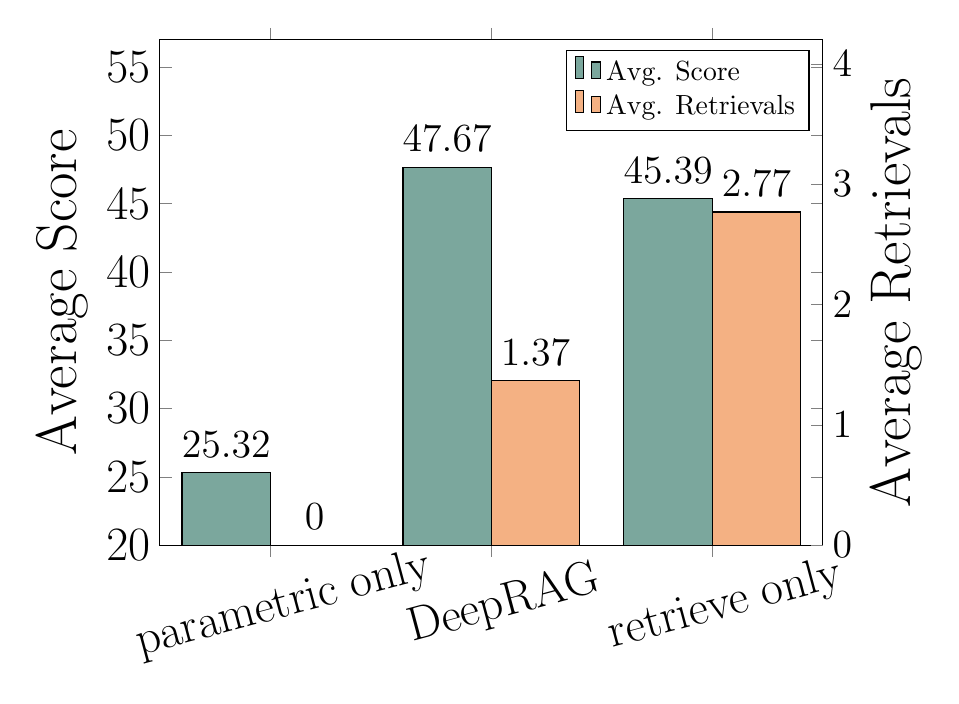
\begin{tikzpicture}

    %=======================%
    %   第一个 axis (左Y轴)
    %=======================%
    \begin{axis}[
        width=10cm,
        height=8cm,
        ybar,
        xmin=0.5, xmax=3.5,
        ymin=20, ymax=57,
        xtick={1,2,3},
        xticklabels={parametric only,DeepRAG,retrieve only},
        ticklabel style={font=\LARGE},
        xticklabel style={
            rotate=15,
            anchor=center,
            yshift=-18
        },
        label style={font=\Large},
        ylabel={Average Score},
        ylabel style={font=\huge},
        bar width=0.4,
        legend style={
            % at={(0.5,1.15)},    % 调整图例位置到图表上方
            anchor=north east,       % 设置锚点为北
            font=\normalsize,
            cells={anchor=west},
        },
    ]

    %------ 左柱: Avg. Score ------%
    % 3 个方法, x=1-0.2=0.8, 2-0.2=1.8, 3-0.2=2.8
    \addplot[
        fill={rgb,255:red,123; green,167; blue,157},
        nodes near coords,
        point meta=y,
        every node near coord/.append style={font=\Large, yshift=2pt}
    ] coordinates {
        (0.8,25.32)
        (1.8,47.67)
        (2.8,45.39)
    };
    \addlegendentry{Avg. Score}

    % 为图例先添加一个条目(不用实际绘制), 代表右柱
    \addlegendimage{fill={rgb,255:red,244; green,177; blue,131}}
    \addlegendentry{Avg. Retrievals}

    \end{axis}

    %==========================%
    %   第二个 axis (右Y轴)
    %==========================%
    \begin{axis}[
        width=10cm,
        height=8cm,
        ybar,
        xmin=0.5, xmax=3.5,
        ymin=0, ymax=4.2,
        axis x line=none,
        axis y line*=right,
        ticklabel style={font=\Large},
        label style={font=\Large},
        ylabel={Average Retrievals},
        ylabel style={font=\huge},
        bar width=0.4,
    ]

    %------ 右柱: Avg. Retrievals ------%
    % x=1+0.2=1.2, 2+0.2=2.2, 3+0.2=3.2
    \addplot[
        fill={rgb,255:red,244; green,177; blue,131},
        nodes near coords,
        point meta=y,
        every node near coord/.append style={font=\Large, yshift=2pt}
    ] coordinates {
        (1.2,0.0)
        (2.2,1.368912773)
        (3.2,2.768780685)
    };

    \end{axis}

\end{tikzpicture}
}
        \caption{Comparative analysis of retrieval strategies: parametric only or retrieve only.}
        \label{fig:analysis1}
    \end{minipage}
    \hfill
    \begin{minipage}[b]{0.66\textwidth}
        \centering
        \begin{minipage}[b]{0.48\textwidth}
            \centering
            \resizebox{\textwidth}{!}{
    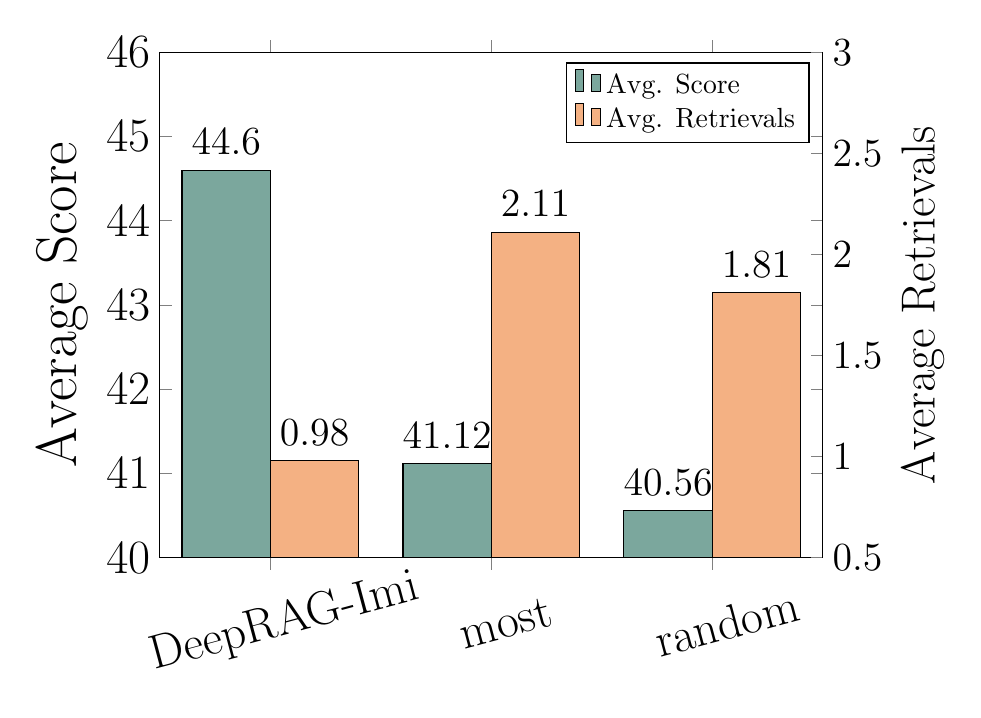
\begin{tikzpicture}
    \begin{axis}[
        width=10cm,
        height=8cm,
        ybar,
        xmin=0.5, xmax=3.5,
        ymin=40, ymax=46,
        xtick={1,2,3},
        xticklabels={DeepRAG-Imi,most,random},
        ticklabel style={font=\LARGE},
        xticklabel style={
            rotate=15,
            anchor=center,     % 让旋转后的文字对齐方式合理
            yshift=-20
          },
        label style={font=\LARGE},
        ylabel={Average Score},
        ylabel style={font=\huge},
        bar width=0.4,
        legend style={
            % at={(0.5,1.15)},    % 调整图例位置到图表上方
            anchor=north east,       % 设置锚点为北
            font=\normalsize,
            cells={anchor=west},
        }
    ]

    \addplot[
        fill={rgb,255:red,123; green,167; blue,157},
        nodes near coords,
        point meta=y,
        every node near coord/.append style={font=\Large, yshift=2pt}
    ] coordinates {
        (0.8,44.60)
        (1.8,41.12)
        (2.8,40.56)
    };
    \addlegendentry{Avg. Score}

    % 在第一个坐标系中添加第二个图例
    \addlegendimage{fill={rgb,255:red,244; green,177; blue,131}}
    \addlegendentry{Avg. Retrievals}

    \end{axis}

    \begin{axis}[
        width=10cm,
        height=8cm,
        ybar,
        xmin=0.5, xmax=3.5,
        ymin=0.5, ymax=3,
        axis x line=none,
        axis y line*=right,
        ticklabel style={font=\Large},
        label style={font=\LARGE},
        ylabel={Average Retrievals},
        ylabel style={font=\LARGE},
        bar width=0.4,
    ]

    \addplot[
        fill={rgb,255:red,244; green,177; blue,131},
        nodes near coords,
        point meta=y,
        every node near coord/.append style={font=\Large, yshift=2pt}
    ] coordinates {
        (1.2,0.98)
        (2.2,2.11)
        (3.2,1.81)
    };

    \end{axis}
    \end{tikzpicture}
}
            % \includegraphics[width=\textwidth]{figure/ablation1.pdf}
            (a)
        \end{minipage}
        \hfill
        \begin{minipage}[b]{0.48\textwidth}
            \centering
            
    \resizebox{\textwidth}{!}{
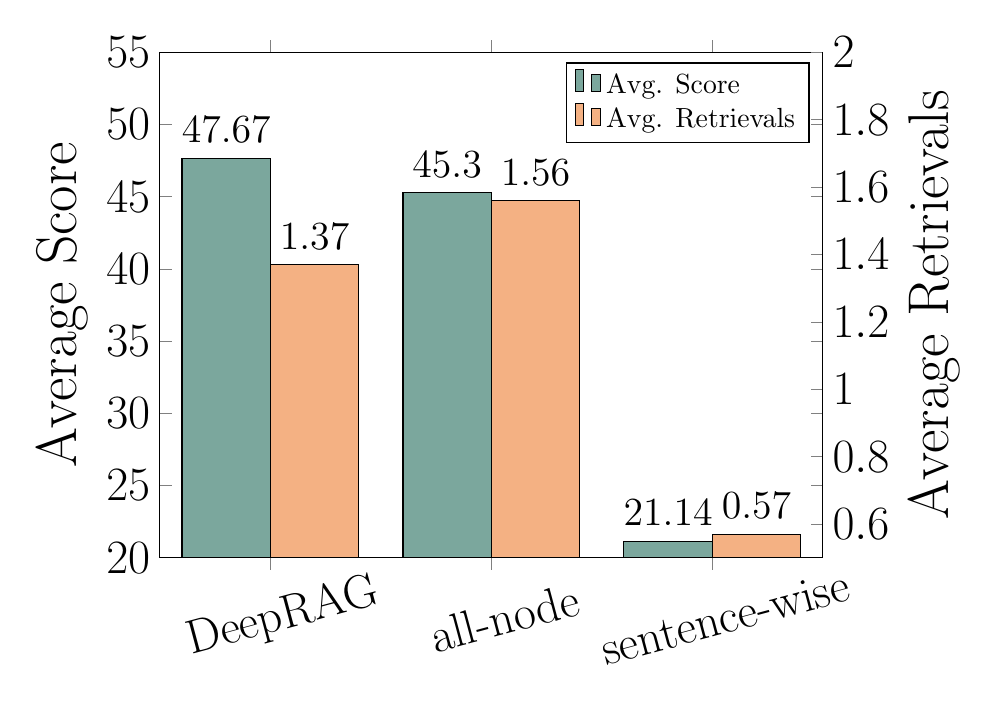
\begin{tikzpicture}

    %=======================%
    %   第一个 axis (左Y轴)
    %=======================%
    \begin{axis}[
        width=10cm,
        height=8cm,
        ybar,
        xmin=0.5, xmax=3.5,
        ymin=20, ymax=55,
        xtick={1,2,3},
        xticklabels={DeepRAG,all-node,sentence-wise},
        ticklabel style={font=\LARGE},     % 刻度字号
        xticklabel style={
            rotate=15,
            anchor=center,
            yshift=-18
        },
        label style={font=\Large},         % 轴标题字号
        ylabel={Average Score},
        ylabel style={font=\huge},
        bar width=0.4,
        legend style={
            % at={(0.5,1.15)},    % 调整图例位置到图表上方
            anchor=north east,       % 设置锚点为北
            font=\normalsize,
            cells={anchor=west},
        }
    ]

    %------ 左柱: Avg. Score ------%
    % 3 个方法, x=1-0.2=0.8, 2-0.2=1.8, 3-0.2=2.8
    \addplot[
        fill={rgb,255:red,123; green,167; blue,157},
        nodes near coords,
        point meta=y,
        every node near coord/.append style={font=\Large, yshift=2pt}
    ] coordinates {
        (0.8,47.67)
        (1.8,45.30)
        (2.8,21.14)
    };
    \addlegendentry{Avg. Score}

    % 为图例先添加一个条目(不用实际绘制), 代表右柱
    \addlegendimage{fill={rgb,255:red,244; green,177; blue,131}}
    \addlegendentry{Avg. Retrievals}

    \end{axis}

    %==========================%
    %   第二个 axis (右Y轴)
    %==========================%
    \begin{axis}[
        width=10cm,
        height=8cm,
        ybar,
        xmin=0.5, xmax=3.5,
        ymin=0.5, ymax=2.0,
        axis x line=none,
        axis y line*=right,
        ticklabel style={font=\LARGE},
        label style={font=\Large},
        ylabel={Average Retrievals},
        ylabel style={font=\huge},
        bar width=0.4,
    ]

    %------ 右柱: Avg. Retrievals ------%
    % x=1+0.2=1.2, 2+0.2=2.2, 3+0.2=3.2
    \addplot[
        fill={rgb,255:red,244; green,177; blue,131},
        nodes near coords,
        point meta=y,
        every node near coord/.append style={font=\Large, yshift=2pt}
    ] coordinates {
        (1.2,1.37)
        (2.2,1.56)
        (3.2,0.57)
    };

    \end{axis}

\end{tikzpicture}
}
            % \includegraphics[width=\textwidth]{figure/ablation2.pdf}
            (b)
        \end{minipage}
        \caption{Average score and retrievals on the ablation study for Imitation Learning and Chain of Calibration. }
        \label{fig:ablation}
    \end{minipage}
\end{figure*}



